% Asset ID: AS1VectorsTikZ-005
% Source: P1-Chp11-Vectors.pdf, Position Vectors slides
% Related lesson section: Core Theory: Position vectors and vector differences; Worked Examples 9 and 10
% Purpose: Show position vectors from the origin and vector difference AB = OB - OA.
\documentclass[tikz,border=8pt]{standalone}
\usepackage{amsmath}
\usepackage{bm}
\usetikzlibrary{arrows.meta,positioning,angles,quotes}
\begin{document}

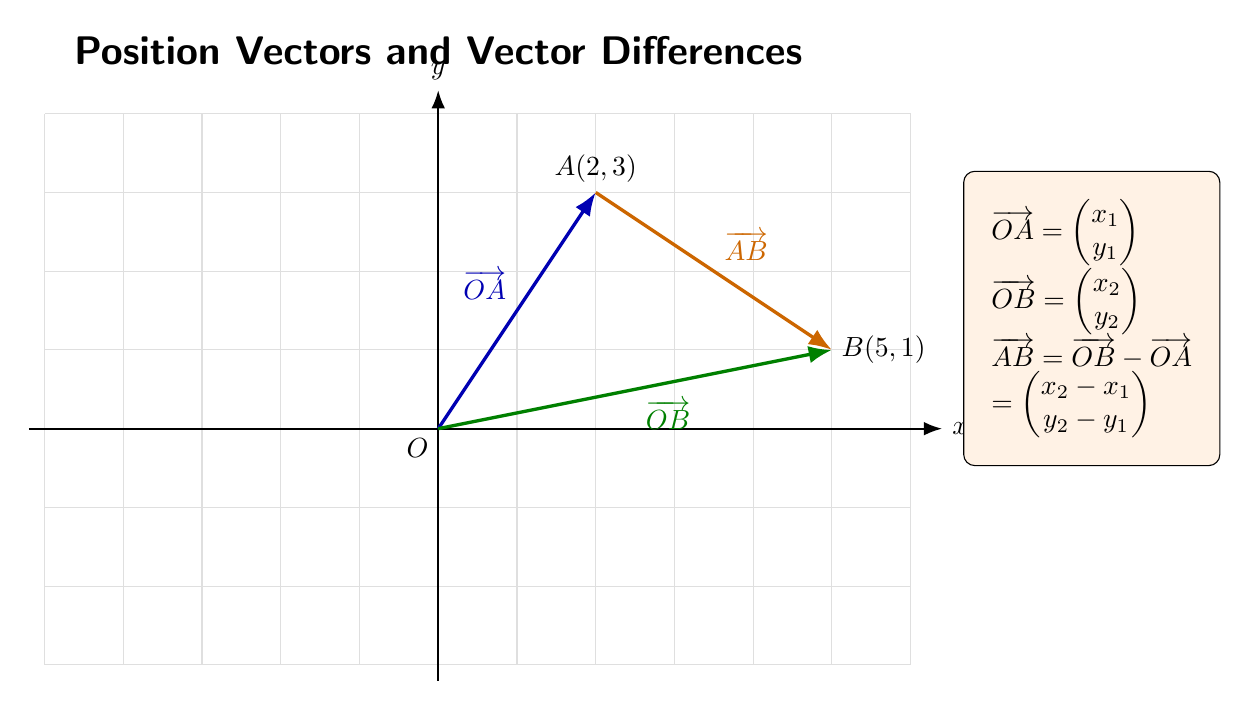
\begin{tikzpicture}[>=Latex,every node/.style={font=\sffamily},oa/.style={->,very thick,blue!70!black},ob/.style={->,very thick,green!50!black},ab/.style={->,very thick,orange!80!black}]
\node[font=\sffamily\bfseries\Large] at (0,4.8) {Position Vectors and Vector Differences};
\draw[step=1,gray!25] (-5,-3) grid (6,4);\draw[->,thick] (-5.2,0)--(6.4,0) node[right] {$x$};\draw[->,thick] (0,-3.2)--(0,4.3) node[above] {$y$};
\coordinate (O) at (0,0);\coordinate (A) at (2,3);\coordinate (B) at (5,1);
\draw[oa] (O)--node[above left] {$\overrightarrow{OA}$}(A);\draw[ob] (O)--node[below right] {$\overrightarrow{OB}$}(B);\draw[ab] (A)--node[above right] {$\overrightarrow{AB}$}(B);
\node[below left] at (O) {$O$};\node[above] at (A) {$A(2,3)$};\node[right] at (B) {$B(5,1)$};
\node[draw,rounded corners,fill=orange!10,align=left,inner sep=10pt] at (8.3,1.4) {$\overrightarrow{OA}=\begin{pmatrix}x_1\\y_1\end{pmatrix}$\\$\overrightarrow{OB}=\begin{pmatrix}x_2\\y_2\end{pmatrix}$\\$\overrightarrow{AB}=\overrightarrow{OB}-\overrightarrow{OA}$\\$=\begin{pmatrix}x_2-x_1\\y_2-y_1\end{pmatrix}$};
\end{tikzpicture}

\end{document}
